% !TEX TS-program = pdflatex
% !TEX encoding = UTF-8 Unicode

% This is a simple template for a LaTeX document using the "article" class.
% See "book", "report", "letter" for other types of document.

\documentclass[11pt]{article} % use larger type; default would be 10pt

\usepackage[utf8]{inputenc} % set input encoding (not needed with XeLaTeX)

%%% Examples of Article customizations
% These packages are optional, depending whether you want the features they provide.
% See the LaTeX Companion or other references for full information.

%%% PAGE DIMENSIONS
\usepackage{geometry} % to change the page dimensions
\geometry{a4paper} % or letterpaper (US) or a5paper or....
% \geometry{landscape} % set up the page for landscape
%   read geometry.pdf for detailed page layout information

\usepackage{graphicx} % support the \includegraphics command and options

% \usepackage[parfill]{parskip} % Activate to begin paragraphs with an empty line rather than an indent

%%% PACKAGES
\usepackage{booktabs} % for much better looking tables
\usepackage{array} % for better arrays (eg matrices) in maths
%\usepackage{paralist} % very flexible & customisable lists (eg. enumerate/itemize, etc.)
%TODO uncomment paralist
\usepackage{verbatim} % adds environment for commenting out blocks of text & for better verbatim
\usepackage{subfig} % make it possible to include more than one captioned figure/table in a single float
% These packages are all incorporated in the memoir class to one degree or another...

\usepackage{float}
\usepackage{tabularx}
\usepackage{color}
\usepackage{xcolor}
\usepackage{listings}
\usepackage{caption}
\usepackage{cite}
\usepackage{hyperref}
\DeclareCaptionFont{white}{\color{white}}
\DeclareCaptionFormat{listing}{\colorbox{gray}{\parbox{\textwidth}{#1#2#3}}}
\captionsetup[lstlisting]{format=listing,labelfont=white,textfont=white}

\newcommand{\myparagraph}[1]{\paragraph{#1}\mbox{}\\}

\def\worksheet#1#2{%
  \begin{center}
  {\large\bf #1} \\
  {\normalsize\bf #2} \\[12pt]
  \begin{footnotesize}
  \input work-sheets-in-latex/#1.tex
  \end{footnotesize}
  \end{center}  
  \vfill}

\renewcommand\appendix{\par
  \setcounter{section}{0}
  \setcounter{subsection}{0}
  \setcounter{figure}{0}
  \setcounter{table}{0}
  \renewcommand\thesection{Appendix \Alph{section}}
  \renewcommand\thefigure{\Alph{section}\arabic{figure}}
  \renewcommand\thetable{\Alph{section}\arabic{table}}
}

%%% HEADERS & FOOTERS
\usepackage{fancyhdr} % This should be set AFTER setting up the page geometry
\pagestyle{fancy} % options: empty , plain , fancy
\renewcommand{\headrulewidth}{0pt} % customise the layout...
\lhead{}\chead{}\rhead{}
\lfoot{}\cfoot{\thepage}\rfoot{}


\newcommand*{\titleGM}{\begingroup 
\hbox{ 
\hspace*{0.1\textwidth} 
\rule{1pt}{\textheight} 
\hspace*{0.05\textwidth} 
\parbox[b]{0.75\textwidth}{ 

{\noindent\Huge\bfseries easyAround}\\[1\baselineskip] % Title
{\large \textit{Knowledge Engineering project}}\\[4\baselineskip] % Tagline or further description
%
{\Large 
\textsc{Claudia Minardi}
\\
\textcolor{gray}{\href{mailto:minardi.claudia@gmail.com}{\emph{minardi.claudia@gmail.com}}} \\\\
\textsc{Marco De Nadai}
\\
\textcolor{gray}{\href{mailto:me@marcodena.it}{\emph{me@marcodena.it}}} \\
\vspace{2.5cm}
} % Author name

\vspace{0.4\textheight} % Whitespace between the title block and the publisher
{\noindent \textbf{Vrije Universiteit} \\ Amsterdam, The Netherlands \\ 2014 }\\[\baselineskip] % Publisher and logo
}}
\endgroup}

\begin{document}
\pagestyle{empty}
\titleGM


\section{Introduction}
This document illustrates the process of the development of an information system according to the CommonKADS~\cite{schreiber2000knowledge} approach. \\
The idea at the base of the project is to build a system capable of assisting a Travel Agent in satisfying the customers. The software must be able to exploit the knowledge of the Travel Agent in order to build a customized itinerary that reflect the desire of the client. \\
To do so, it is necessary to have precise knowledge rules embedded inside the system itself: this can be done by building a series of models that will constitute the core structure of the software. \\
The final piece of software, namely \textit{easyAround} will be able to:
\begin{itemize}
\item Classify customers according to their age and physical capabilities;
\item Gather information on each customer's preferences and personal taste;
\item Gather specific information on each customer's desire for a specific trip;
\item Propose to each customer an ideal trip, based on the gathered information;
\item Let the customers revise and personalize their own itinerary;
\end{itemize}
The target domain of the software resides inside one single city: the final itineary will be composed of locations to be visited inside that particular city, according to a standard timetable possessed by the Travel Agency. \\
The target user of the software is the Travel Agent appointed with the task of creating cusomized itineraries for clients who travel alone or accompanied by children.
\newpage
\section{Context Knowledge}
\worksheet{OM-1}{Identifying knowledge-oriented problems and
opportunities in the organization}
\worksheet{OM-2}{Description of organizational aspects that
have an impact on and/or are affected by chosen knowledge solutions}
\begin{figure}[H]
\centering
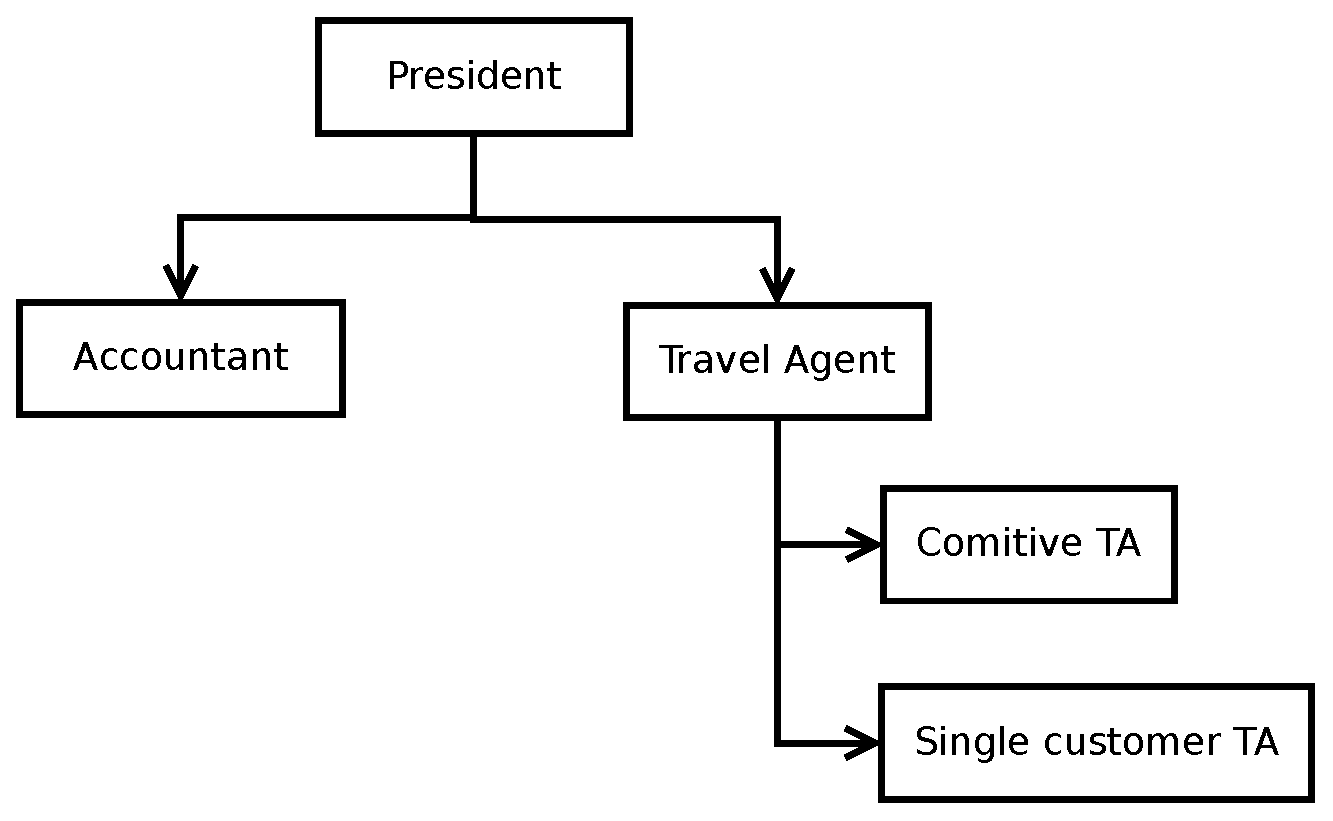
\includegraphics[width=10cm]{images/azienda.eps}
\caption{Organization structure}
\label{fig:orgStructure}
\end{figure}
\begin{figure}[H]
\centering
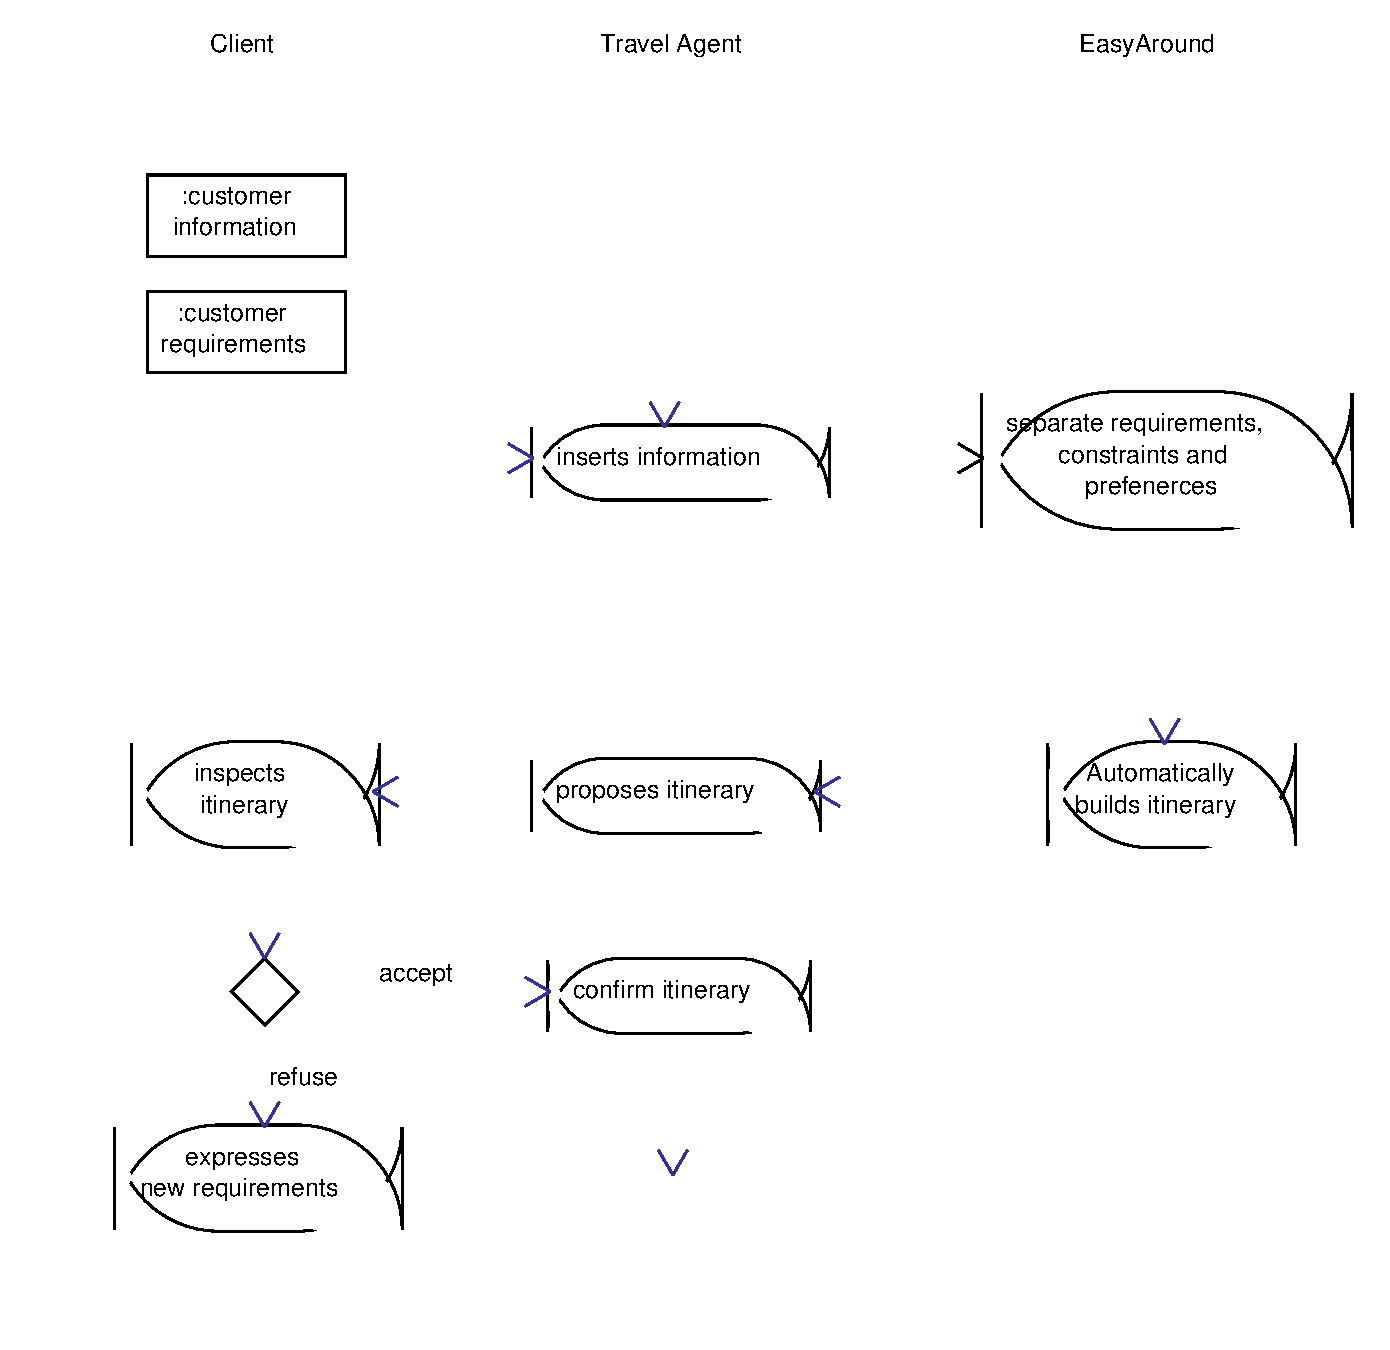
\includegraphics[width=\textwidth]{images/activity.eps}
\caption{Organization process}
\label{fig:orgProcess}
\end{figure}
\newpage
\worksheet{OM-5}{Checklist for the feasibility decision
document}
\worksheet{TM-1}{Refined description of the tasks within the
target process}
\worksheet{TM-2}{Specification of the knowledge employed for a
task, and possible bottlenecks and areas for improvement}
\worksheet{AM-1}{Agent specification according to the
CommonKADS agent model}

\clearpage
\section{Task Knowledge}

\begin{figure}[h]
\centering
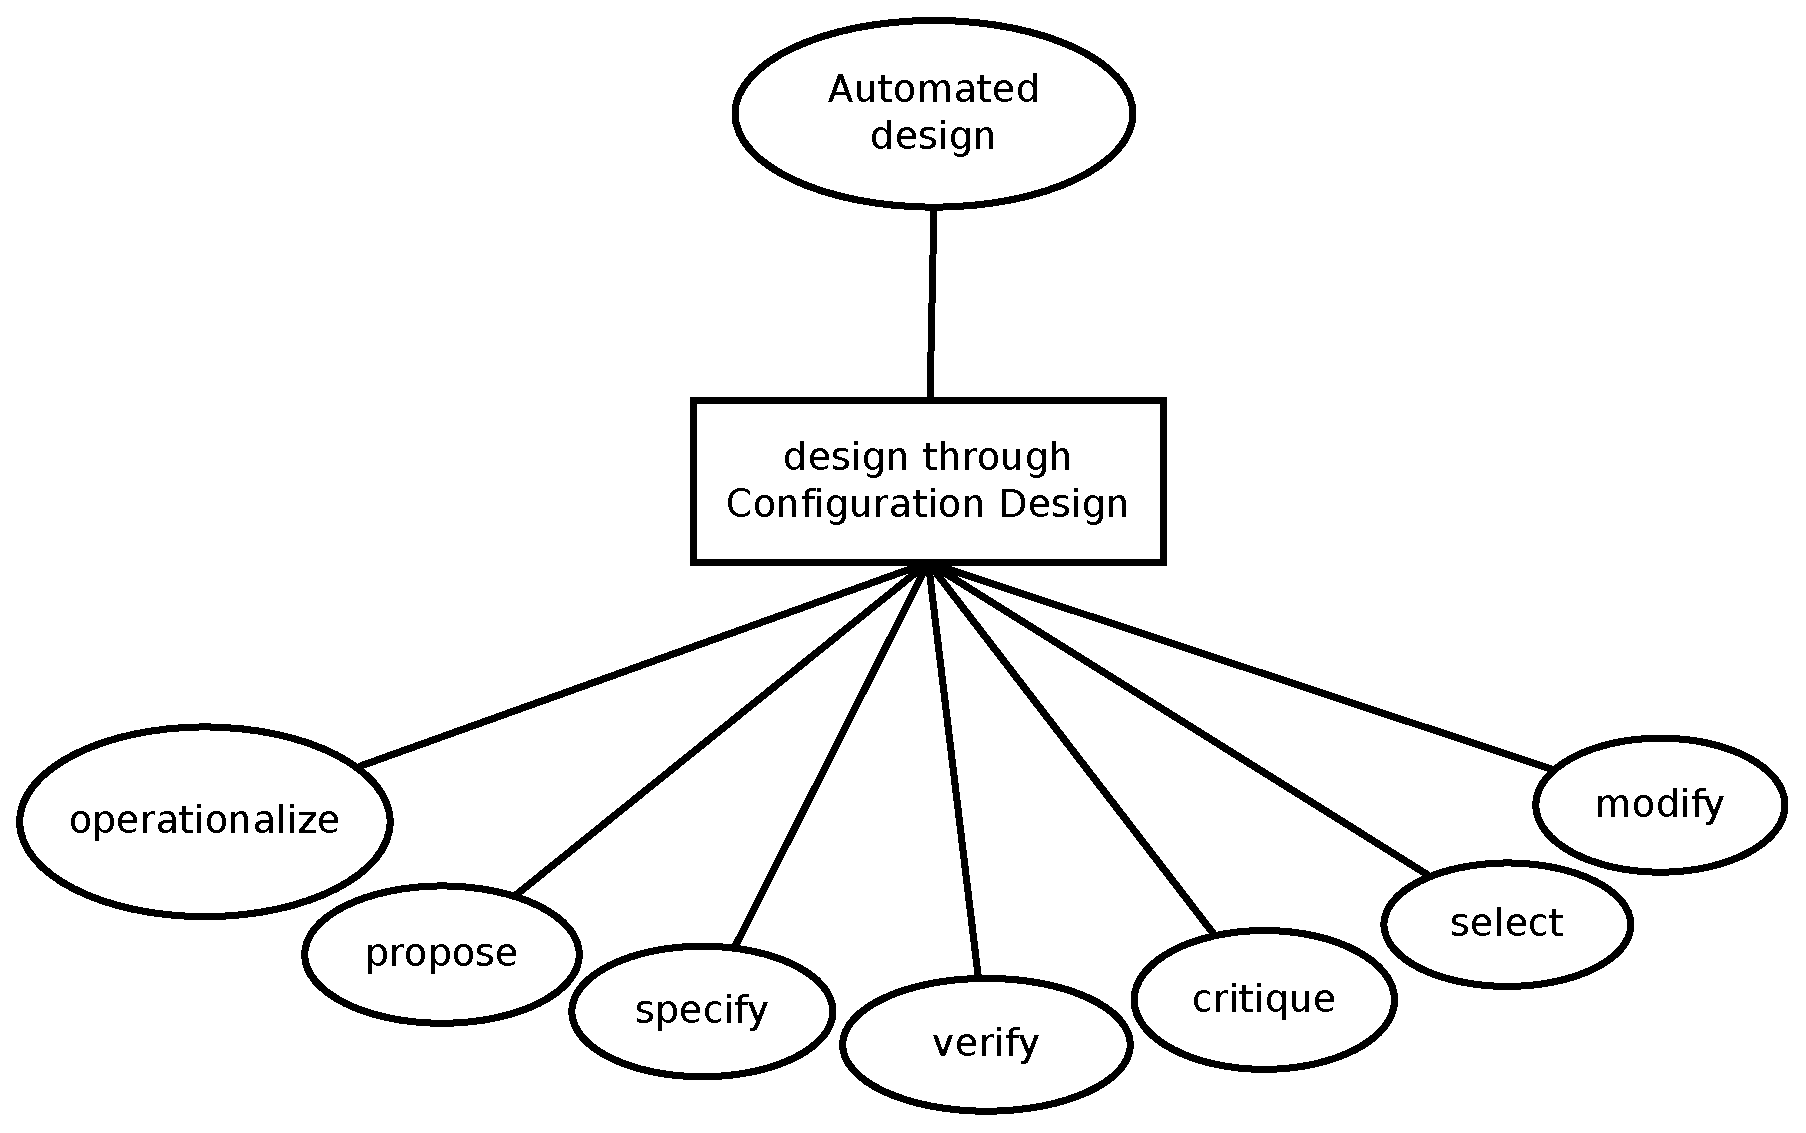
\includegraphics[height=7cm]{images/task_knowledge.eps}
\caption{Task knowledge}
\label{fig:taskknowledge}
\end{figure}

The ``propose and revise" method for configuration design presented in its original form in the textbook for the course has been slightly modified to obtain a method that reflects the needs of our software. The \textit{WHILE} loop to revise the the design has been postponed from a state of \textit{propose} to a state of \textit{verify}, and the internal \textit{REPEAT UNTIL} loop to select the actions has been integrated in the outer cycle. This way the method reflects exactly the intended steps to be realized in the software. 

\begin{lstlisting}[label=Task,caption=Task and task method description,breaklines=true]
TASK automated-design;
  ROLES:
    INPUT: request: "request for the design";
    OUTPUT: itinerary: "the resulting design";
END TASK configuration-design;

TASK-METHOD propose-and-revise;
  REALIZES: automated-design;
  DECOMPOSITION:
    INFERENCES: operationalize, propose, specify, verify, critique, select, modify;
  ROLES:
    INTERMEDIATE:
      preferences-and-requirements: "requirements and preferences to be preferably fulfilled";
      constraints: "requirements that have to be fulfilled";
      skeletal-design: "set of slots to be filled";
      proposal: "a possible compilation of the skeletal-design";
      customer-input: "set of new requirements or constraints";
      violation: "new constraints violated by the current design";
      truth-value: "boolean indicating the result of the verification";
      action-list: "ordered list of possible repair (fix) actions";
      action: "a single repair action";
      itinerary: "a new possible compilation of the skeletal-design";
  CONTROL-STRUCTURE:
    operationalize(request -> preferences-and-requirements + constraints);
    specify(request -> skeletal-design);
    propose(constraints + preferences-and-requirements + skeletal-design -> proposal);
    itinerary := proposal ADD itinerary;
    WHILE verify(customer-input + itinerary -> truth-value + violation) IS truth-value == false DO
      critique(violation + itinerary -> action-list)
      select(action-list -> action)
      modify(itinerary + action -> itinerary)
      verify(itinerary + customer-input -> truth-value + violation);
    END WHILE
END TASK-METHOD propose-and-revise;
\end{lstlisting}

\clearpage
\section{Inference Knowledge} \label{sec:inference}

As inference model we use a modified version of the Configuration design template, because given predefined components we need to find and assembly that satisfies the requirements. The inference model deriving from this task can be found in Figure~\ref{fig:inference}. \\
The standard inference model for the configuration design template (propose and revise) has been modified to better express the needs of our software, in a way that the system interacts directly with the client a second time right after the proposal phase: 
\begin{itemize}
\item Requirements have been transformed in Request
\item Soft and hard requirements have been transformed in ``preferences and requirements'' and ``constraints'' respectively
\item Extension has been changed into ``proposal''
\item Verify requires the direct input of the customer, since it's a verification of subjective correctness more than a verification of constraint violation. 
\item Design has been changed int ``itinerary'' for coherency purposes.
\end{itemize}
It has to be noted that the subsystem building the proposal, in the implementation of the system, does not permit a constraint violation, so the verification of the constrait has been removed because redundant.

\begin{figure}[h]
\centering
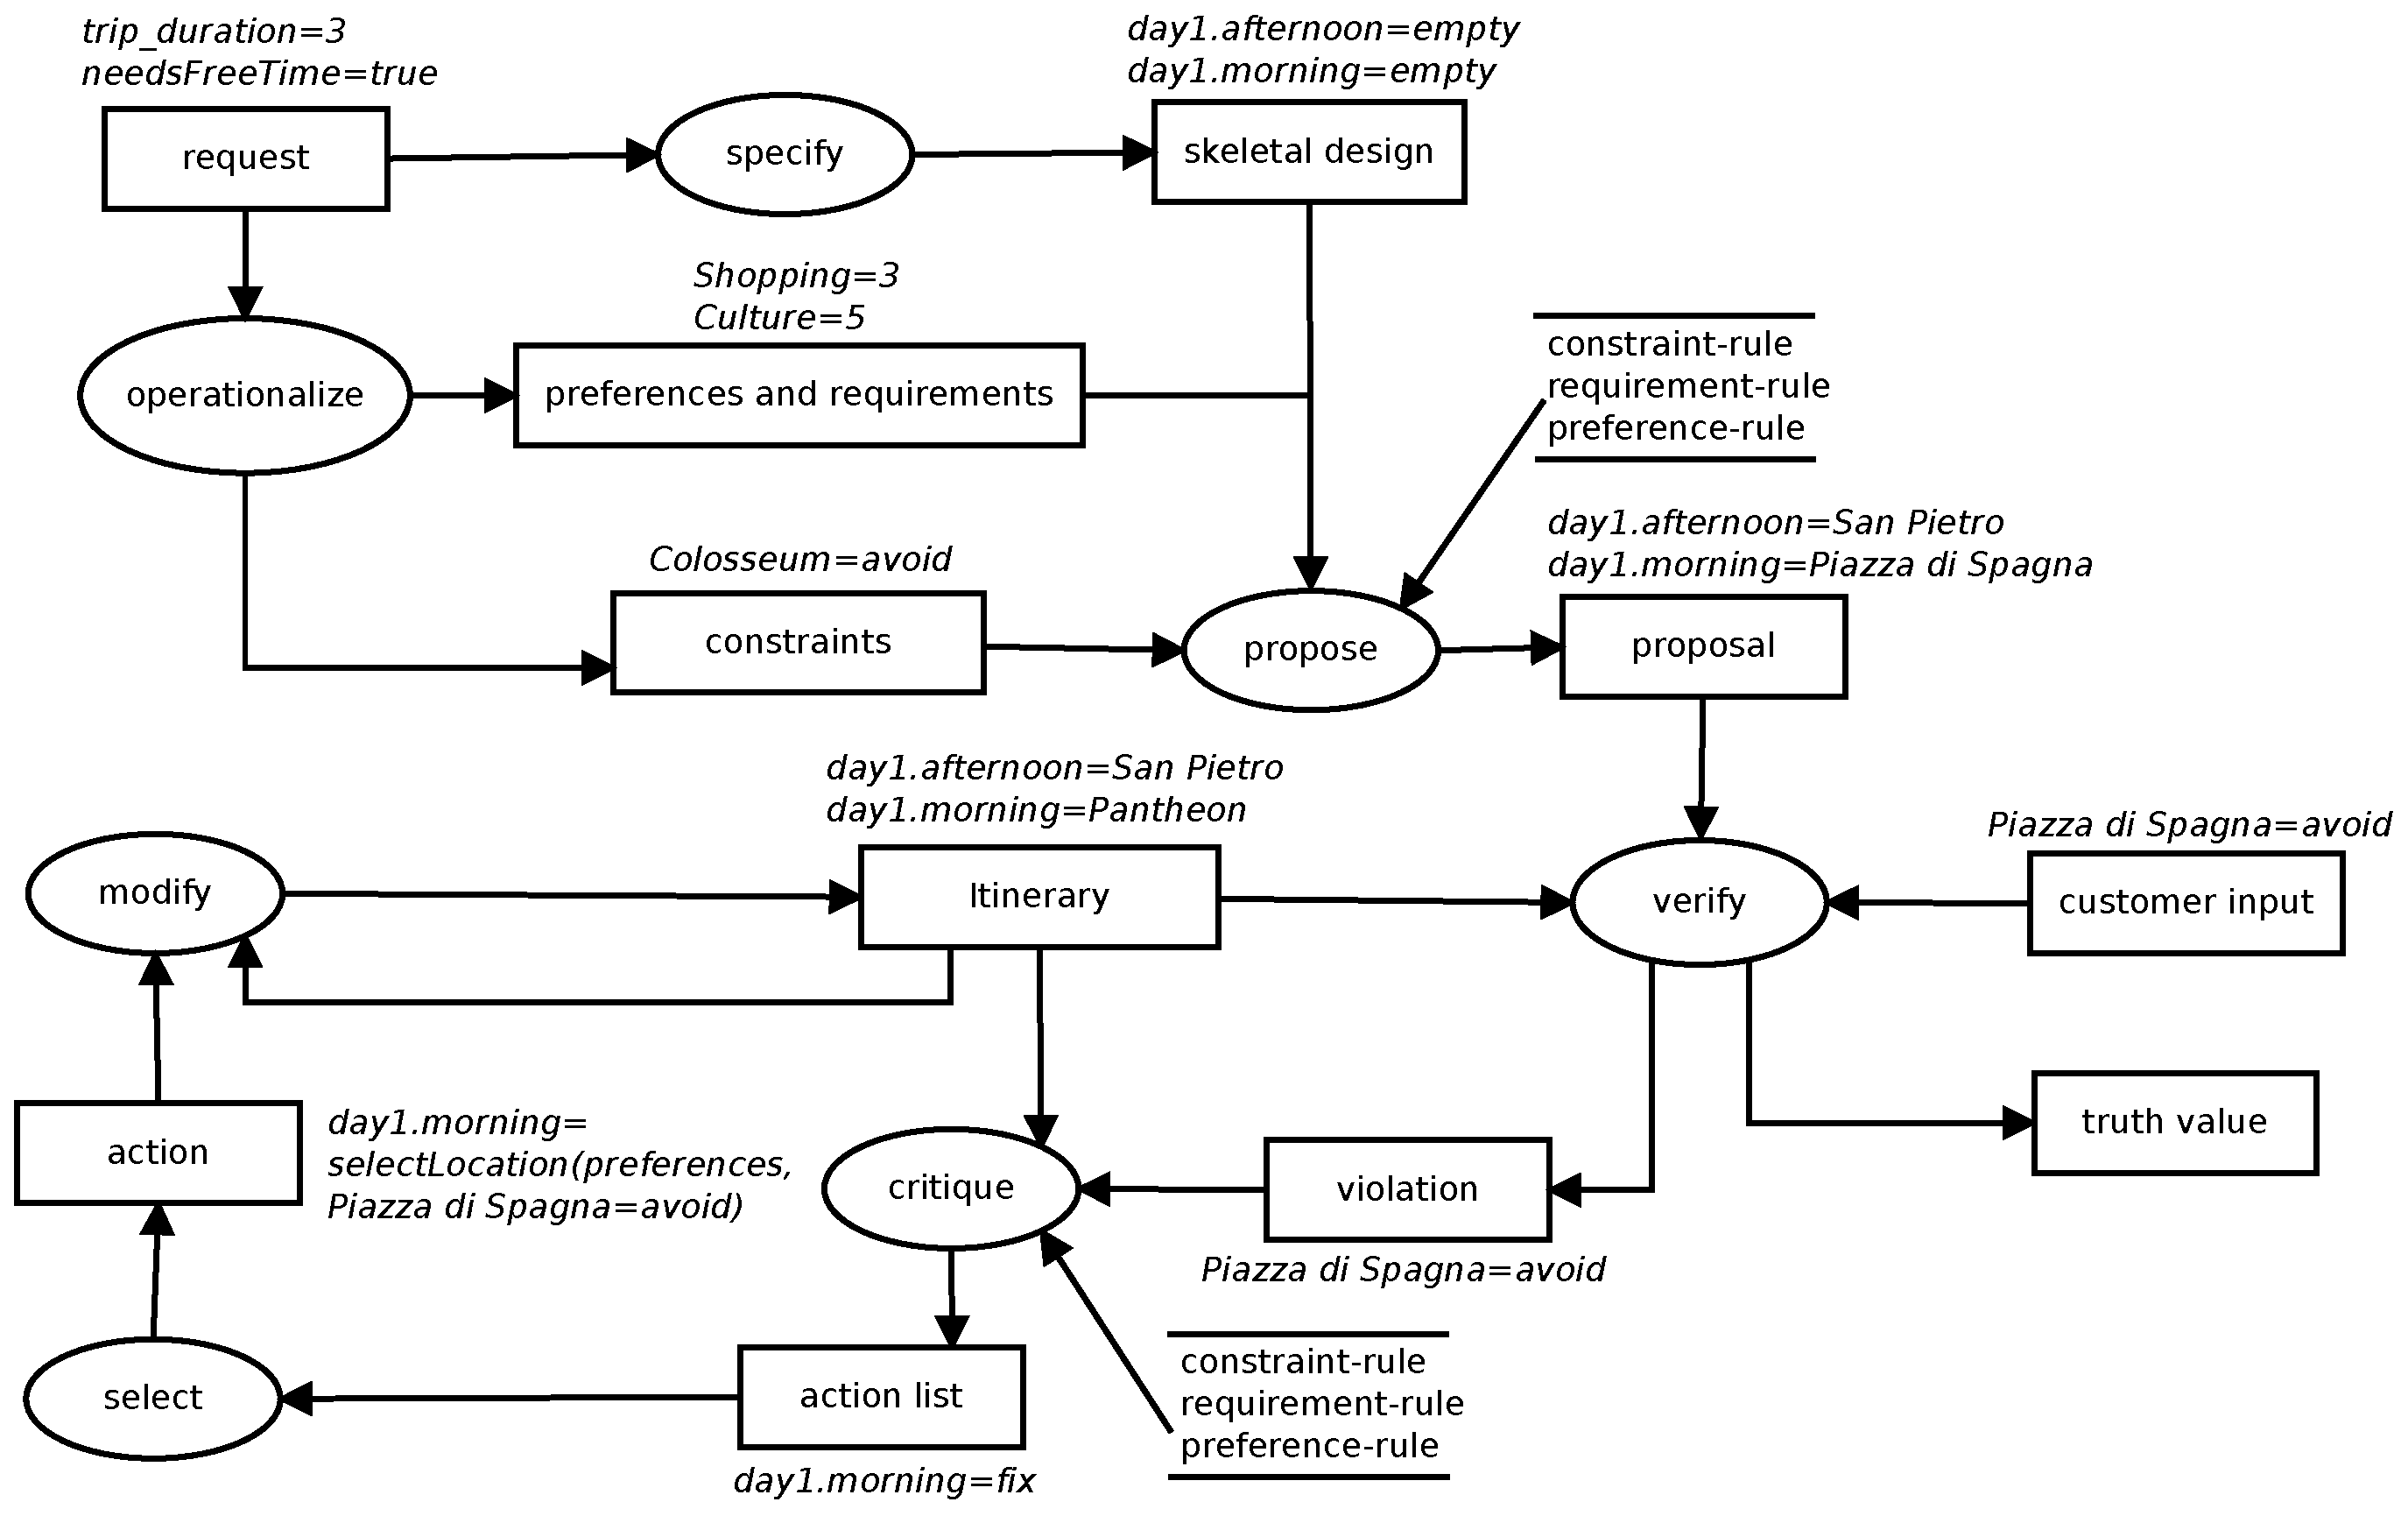
\includegraphics[width=\textwidth]{images/inference.eps}
\caption{Inference structure}
\label{fig:inference}
\end{figure}

\noindent
\begin{tabular}{|p{2.5cm}|p{2.5cm}|p{3cm}|p{6cm}|}
  \hline
Inference		& Input	& Output 	& Description \\ \hline \hline
specify		& request	& skeletal design		& the function builds the default skeletal design: the basic structure of a trip where each day is composed of: morning, afternoon, evening and meal.
\\ \hline 
   operationalize	& needs of the customers		& preferences, requirements, constraints	& the needs and desires are translated into preferences ("I would like to have time for shopping and visit many cultural places. I am not interested so much in food places"), requirements ("I want a quiet trip") and contraints ("In Rome I want to visit the \emph{Colosseum} and avoid \emph{Piazza di Spagna}"). 
\\ \hline
propose	& preferences and requirements, skeletal design and constraints		& filled skeletal design	& fill the slots of the skeletal design with locations that fits the preferences and requirements.
\\
\hline
verify		& proposal and customer input	& -	& it submits the proposal to the TA allowing them to gather the client's critiques.
\\ \hline
select 	& fix actions list		& fix action		& It simply selects an action from the fix actions list generated by the critique function.
\\ \hline
modify	& itinerary design, fix action		& itinerary		& it applies the fix actions to the proposal.
\\ \hline
critique	& itinerary and violations	& fix actions list		& it creates a series of actions which will adjust the itinerary according to the new set of contraints, contained into the violations.
\\ \hline
\end{tabular}

\clearpage
\section{Domain knowledge}

\subsection{Domain schema} \label{sec:domain}
The domain schema can be found in Figure~\ref{fig:ClassDiagram}

\begin{figure}[h]
\centering
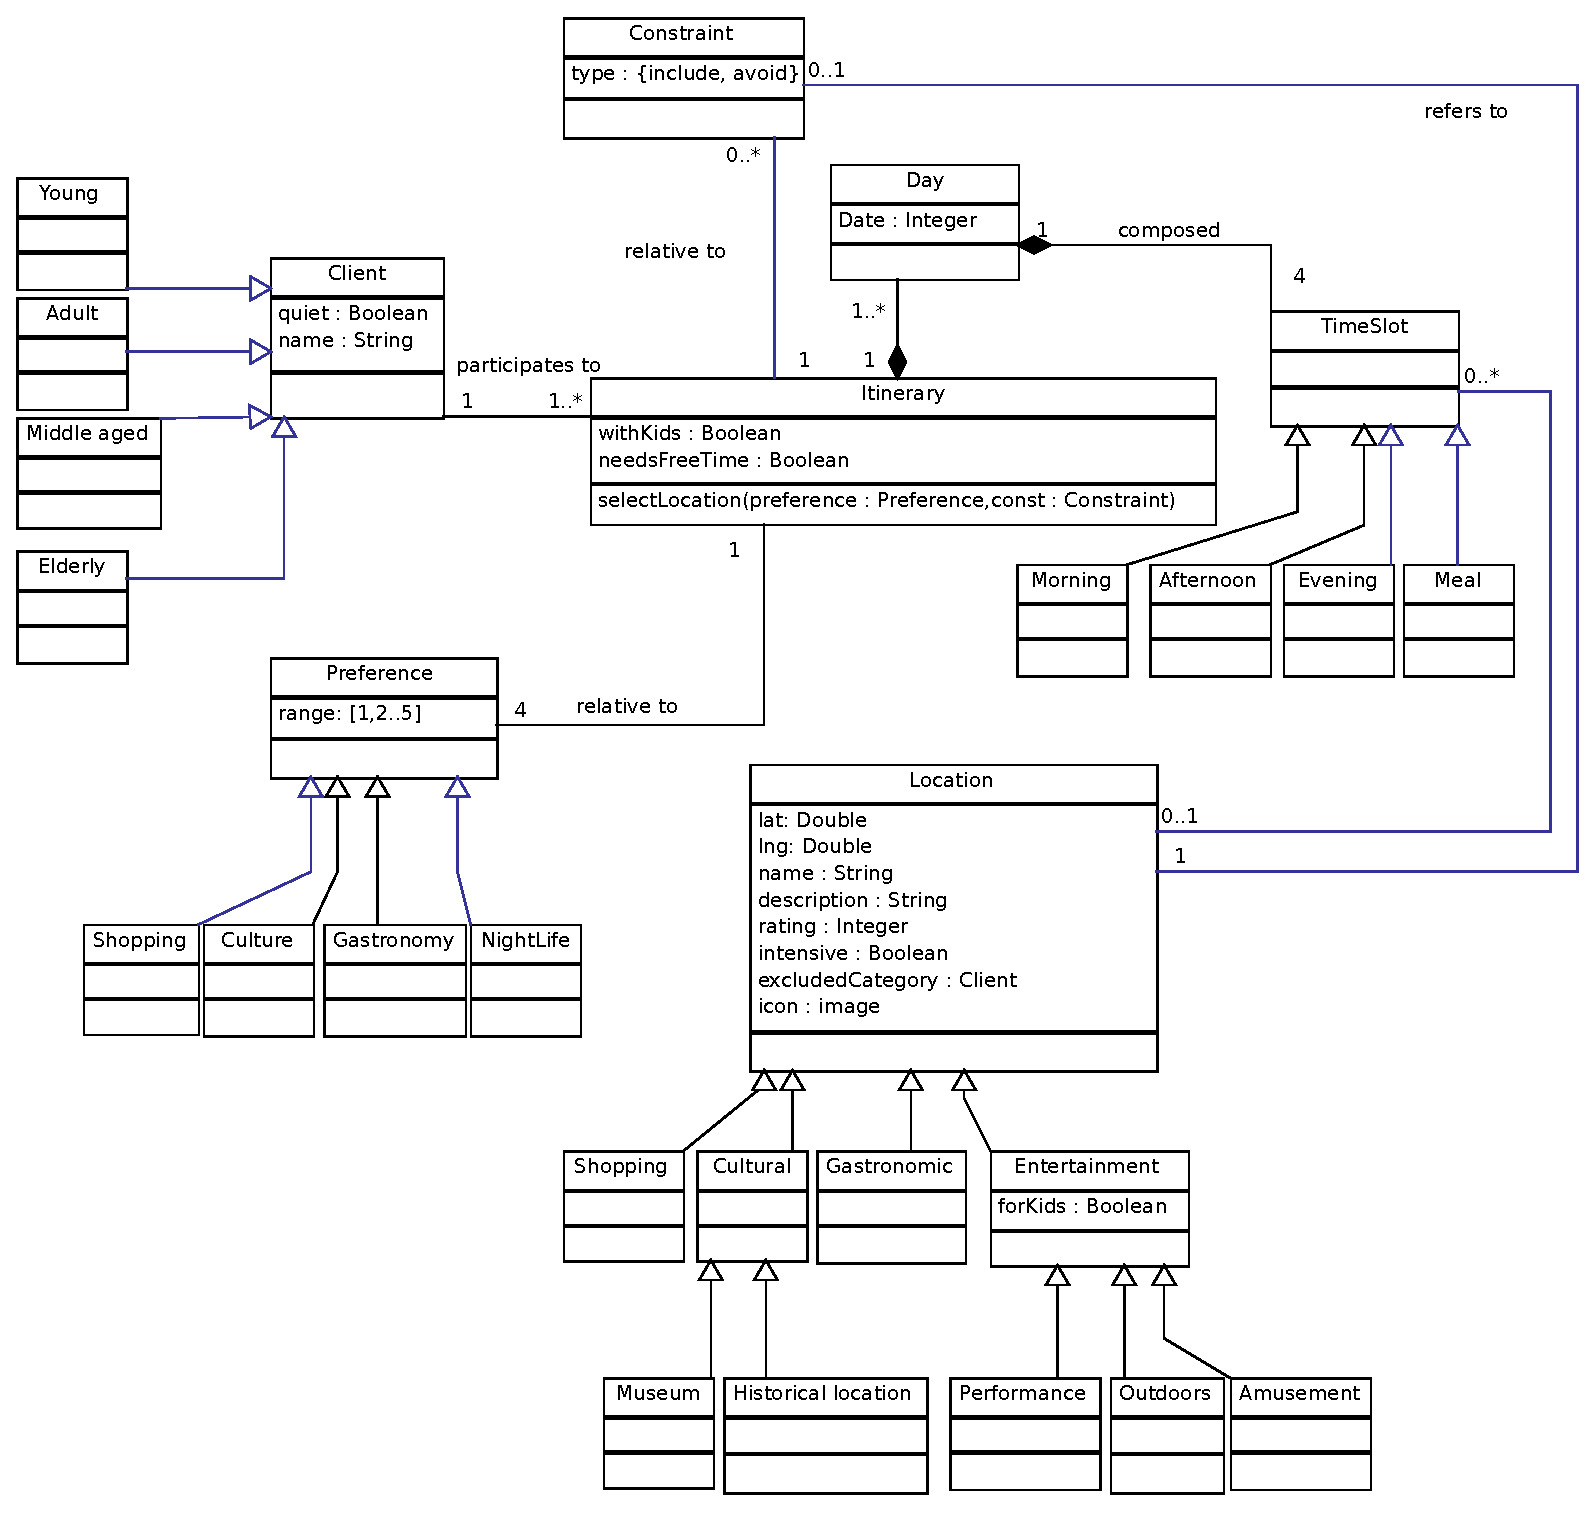
\includegraphics[width=\textwidth]{images/new_domain.eps}
\caption{Domain schema}
\label{fig:ClassDiagram}
\end{figure}

This schema seems complicated, for this reason every model is explained in the following list:
\begin{description}
  \item[Client] \hfill \\
  The client who goes to the travel agency. He can express preferences for a quiet enviroment. The clients are categorized by their age to avoid unsuitable locations (ex: elderly people in a climbing location).

  \item[Preference] \hfill \\
  Each client needs to specify a list of preferences, valued from 1 to 5, where 1 is ``I'm not so interested" and 5 is ``I'd love to do it!". These preferences are related to the itinerary we want to create, consequently if the same clients wants to create another itinerary, it will specify again all the preferences he wants in this second trip.
  \item[Constraint] \hfill \\
  Each client needs to specify a list of contraints that have to be fulfilled. As well as the \emph{Preference}, they are related to the single itinerary.
  \item[Itinerary] \hfill \\
  This represents the itinerary we want to create. It is composed of a fixed number of \emph{Day} and it is related to a \emph{Client} who has specified his own list of \emph{Constraint} and \emph{Preference}. If the itinerary includes kids, the system needs to select some \emph{Location} that could entertain them. This is a requirement as the \emph{needsFreeTime} attribute, which specifies that the clients needs to have some time not allocated by the TA.\\
The method \emph{selectLocation} takes a list of \emph{Preference} and produces a list of \emph{Location} that could fit this preferences. 
  \item[Day] \hfill \\
  This describes a day of the itinerary.
  \item[Timeslot] \hfill \\
  A timeslot is a fixed part of a day. The division of the day came from the expert interview.
\item[Location] \hfill \\
  This model represents the point of interests that a customer could visit. The attribute \emph{rating} describes the quality of this place, \emph{intensive} describes if the place is not for quite people and \emph{excludedCategory} specifies if a client category is not suitable for the location (ex: elderly people in a climbing location).
\end{description}

\subsection{Domain mapping}
\noindent
\begin{tabularx}{\textwidth}{| X | X | X | X |}
\hline 
\textbf{Knowledge Role} & \textbf{Type} & \textbf{Domain Mapping}
\\ \hline \hline
request    &   dynamic  & Client
\\ \hline
skeletal design  & static    & Timeslot
\\ \hline
preferences and requirements  & dynamic    & Client, Itinerary, Preference
\\ \hline
constraints  & dynamic    & Constraint
\\ \hline
customer input  & dynamic    & Constraint
\\ \hline
proposal  & dynamic    & Itinerary
\\ \hline
itinerary  & dynamic    & Itinerary
\\ \hline
violation  & dynamic    & Constraint, Location %TODO: CONTROLLARE SCHEMA
\\ \hline
constraint-rule  & static    & Constraint
\\ \hline
preference-rule  & static    & Preference
\\ \hline
requirement-rule  & static    & Client, Itinerary
\\ \hline
\end{tabularx}

\subsection{Rule types}\label{sec:rules}

\begin{lstlisting}[label=Rules,caption=Rules,breaklines=true]
RULE TYPE constraint-rule;
    DESCRIPTION: "rule stating the relation between client and the choice for a location in the itinerary, by means of defining strict boundaries that must be respected.";
ANTECEDENT: Client;
CONSEQUENT: Itinerary;
CONNECTION-SYMBOL: restricts;
END RULE-TYPE constraint-rule;

RULE TYPE requirement-rule;
    DESCRIPTION: "rule stating the relation between the client and the choice for a location in the itinerary, by means of defining boundaries that should be respected.";
ANTECEDENT: Client;
CONSEQUENT: Itinerary;
CONNECTION-SYMBOL: requires;
END RULE-TYPE requirement-rule;

RULE TYPE preference-rule;
    DESCRIPTION: "rule stating the relation between the client and the choice for a location in the itinerary, by means of defining preferences that could be satisfied with probability X (calculated on the input values) .";
ANTECEDENT: Client;
CONSEQUENT: Itinerary;
CONNECTION-SYMBOL: prefers-with-probability;
END RULE-TYPE preference-rule;
\end{lstlisting}


\noindent
Here are presented also some example in order to better understand all the rule types.

\begin{lstlisting}[label=Rules,caption=The client wants to include a destination into the itinerary.,breaklines=true,mathescape=true]
client.constraint.location.name$=$A AND client.constraint.type$=$include
RESTRICTS
$\exists$itinerary.day.timeslot, timeslot.location.name$=$A;
\end{lstlisting}


\begin{lstlisting}[label=Rules,caption=The client is a quite person,breaklines=true,mathescape=true]
client.quiet=true, client.needsFreeTime=true
REQUIRES
itinerary.day.timeslot.location, location.intensive=false;
itinerary.day.timeslot, timeslot.location=NULL;
\end{lstlisting}




\begin{lstlisting}[label=Rules,caption=The client expresses four preferences with four ranges (from 1 to 5). The method selectLocation will compose the itinerary selecting the locations that fits the preferences. For example it could select 3 shopping\, 1 gastronomy and 1 cultural locations.,breaklines=true,mathescape=true]
Var A, B, C, D: client.preference;
Var E: client.constraint;
A.type=shopping AND A.range=x
B.type=cultural AND B.range=y
C.type=gastronomy AND C.range=w
D.type=nightlife AND D.range=z
E.type = avoid AND E.location = Colusseum
PREFERS-WITH-PROBABILITY
$\forall$itinerary.day.timeslot, timeslot.location=selectLocation(A, B, C, D, E);
\end{lstlisting}

\subsection{Knowledge Base}

The Knowledge base can be seen in Figure~\ref{fig:knowledgebase}.
In the model it is shown the relation between instances of the types specified in the domain schema, according to the rules used to build the system.

\begin{figure}[H]
\centering
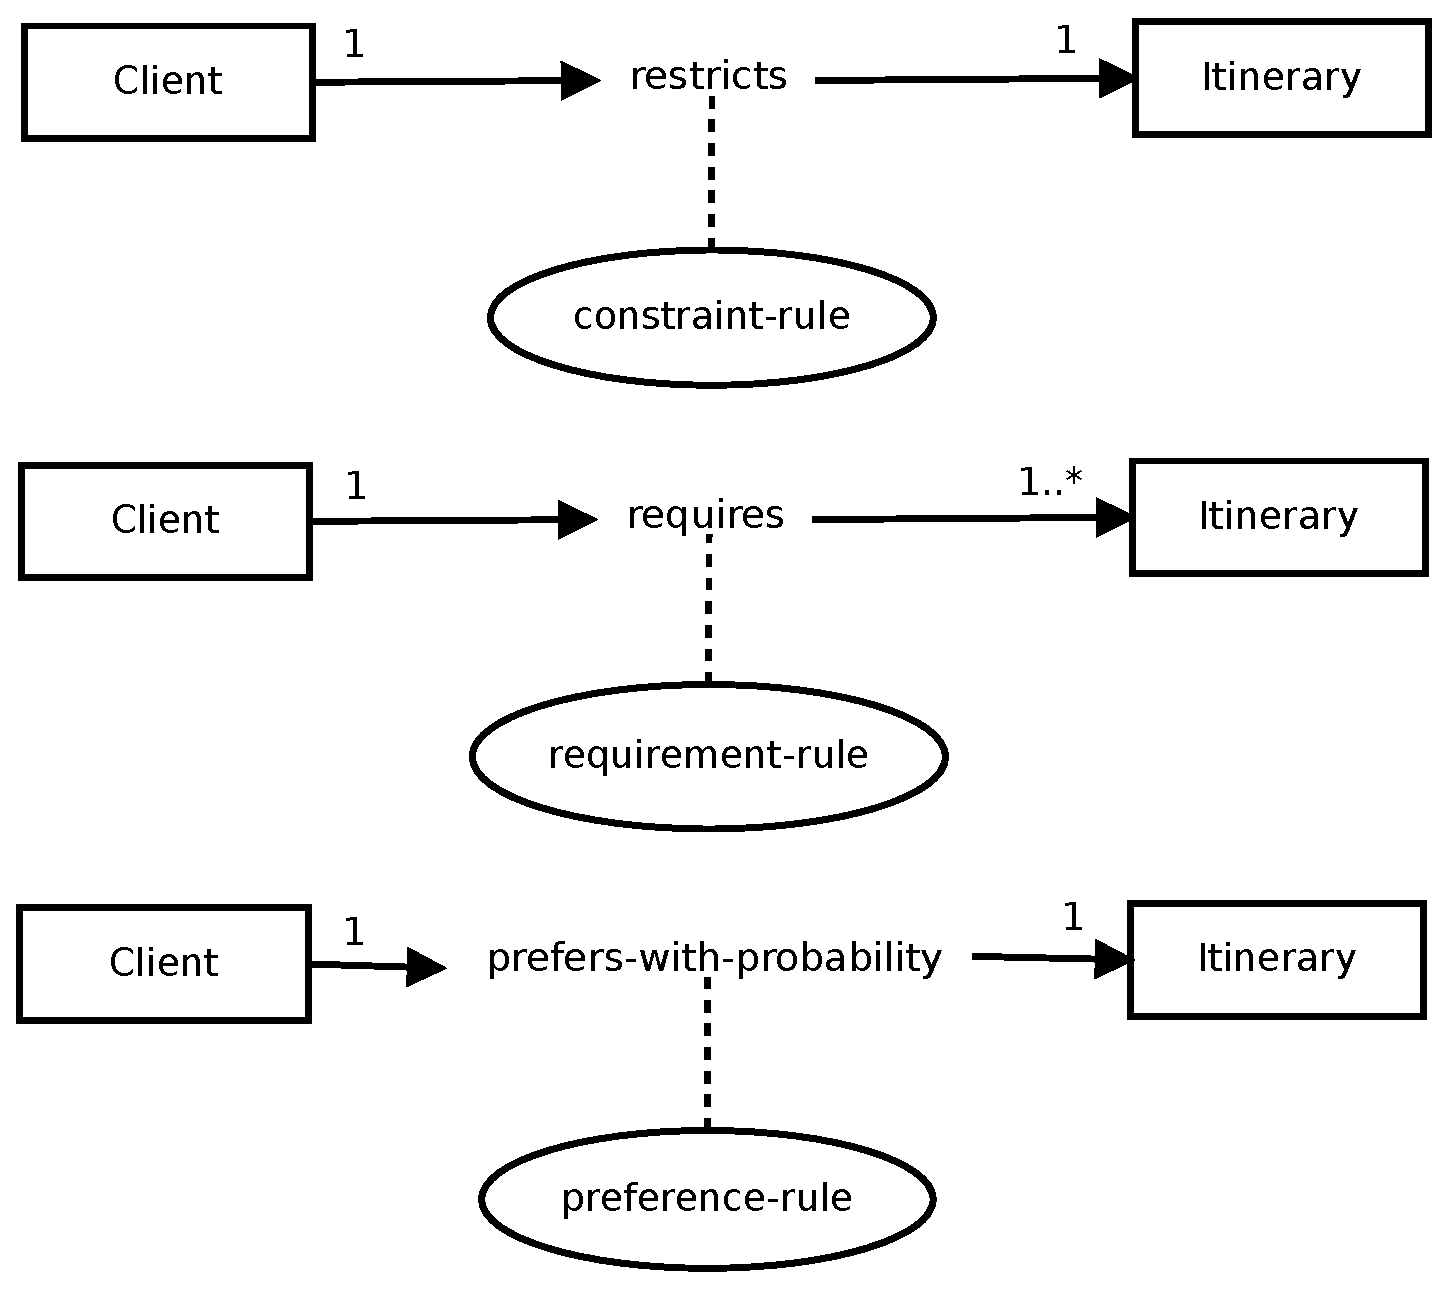
\includegraphics[height=7cm]{images/knowledge_base.eps}
\caption{Knowledge base}
\label{fig:knowledgebase}
\end{figure}



\section{Scenarios}

\subsection{Scenario 1}

Rose, a 76 years old lady would like to visit Rome for three days with her nephew John who is ten years old. She would like to have her trip planned but with the possibility to explore the city on her own. 

\subsubsection{Interview}

\begin{description}
  \item[In a scale from one to five, how do you enjoy shopping?] \hfill \\
  I really love to do shopping, so five!
  \item[In a scale from one to five, how do you enjoy cultural places?] \hfill \\
  I am going to Rome, so four!
  \item[In a scale from one to five, how do you enjoy nightlife?] \hfill \\
  Have you looked at me? 1!
  \item[In a scale from one to five, how much would you like to try new restaurants?] \hfill 
  I guess... I don't know, 3?
  \item[Is there anything that you'd absolutely like to see?] \hfill \\
  Yes, I've never seen the Colosseum.
  \item[Is there anything that you have already seen or don't want to see?] \hfill \\
  Not really, everything is fine.
\end{description}

The travel agent while is interviewing the customer, inserts the acquired data into the system through graphic interface.

\subsubsection{Operazionalize}
The system once it receives the request divides them into three categories: requirements, preferences and constraints.

\begin{lstlisting}[breaklines=true,mathescape=true]
REQUIREMENTS:
  client.quiet = true
  itinerary.withKids = true
  itinerary.needsFreeTime = true
  VAR a,b,c: day;
  a.date = "14/05/2014"
  b.date = "15/05/2014"
  c.date = "16/05/2014"
PREFERENCES:
  VAR a,b,c,d : preference;
  a.type = shopping
  a.range = 5
  b.type = culture
  b.range = 4
  c.type = nightlife
  c.range = 1
  d.type = gastronomy
  d.range = 3
CONSTRAINTS:
  constraint.location.name = Colosseum
  constraint.type = include
\end{lstlisting}

\subsubsection{Specify}
The system reads the request and compiles the skeletal design, an empty itinerary containing only the structure of the days.

\begin{lstlisting}[breaklines=true,mathescape=true]
REQUIREMENTS:
  VAR a,b,c: day;
  a.date = "14/05/2014"
  b.date = "15/05/2014"
  c.date = "16/05/2014"
SKELETAL-DESIGN:
  NEW-ITINERARY(a.date, c.date)
\end{lstlisting}

\subsubsection{Propose}
The system processes the request using the knwoledge rules and returns a first version of the itinerary.

\begin{lstlisting}[breaklines=true,mathescape=true]
ITINERARY:
  VAR a,b,c: day;
  a.date = "14/05/2014"
  b.date = "15/05/2014"
  c.date = "16/05/2014"
  a.morning = Colosseum
  a.afternoon = Shopping mall "I gladiatori"
  a.meal = Parolaccia
  a.evening = Fontana di Trevi
  b.morning = Villa Borghese
  b.afternoon = Outlet shoes Roma
  b.meal = Pizzeria da Matteo
  b.evening = Piazza di Spagna
  c.morning = EMPTY
  c.afternoon = EMPTY 
  c.evening = Piazza del Popolo
  
\end{lstlisting}

\subsubsection{Verify}
The system passes the itinerary to the TA through the GUI. The TA asks the Client for a confirmation or the need for modification.

\begin{description}
  \item[This is a possible itinerary, do you have any modifications you want to do?] \hfill \\
  Yes please, I don't need shoes.
\end{description}

\subsubsection{Critique}
Based on the Client feedback, the system builds an action list of modifications

\begin{lstlisting}[breaklines=true,mathescape=true]
ACTION-LIST:
  contraint.location = Outlet shoes Roma
  constraint.type = avoid
  
\end{lstlisting}

\subsubsection{Select}
The system chooses one action at the time for the itinerary to be modified

\begin{lstlisting}[breaklines=true,mathescape=true]
ACTION:
  contraint.location = Outlet shoes Roma
  constraint.type = avoid
  
\end{lstlisting}

\subsubsection{Modify}
The system modifies the itinerary accordingly to the selected action.

\begin{lstlisting}[breaklines=true,mathescape=true]
ITINERARY:
  VAR a,b,c: day;
  a.date = "14/05/2014"
  b.date = "15/05/2014"
  c.date = "16/05/2014"
  a.morning = Colosseum
  a.afternoon = Shopping mall "I gladiatori"
  a.meal = Parolaccia
  a.evening = Fontana di Trevi
  b.morning = Villa Borghese
  b.afternoon = Le Piramidi
  b.meal = Pizzeria da Nando
  b.evening = Piazza di Spagna
  c.morning = EMPTY
  c.afternoon = EMPTY 
  c.meal = EMPTY
  c.evening = Piazza del Popolo
  
\end{lstlisting}

\subsubsection{Verify}
The system passes the itinerary to the TA through the GUI. The TA asks the Client for a confirmation or the need for modification.

\begin{description}
  \item[This is a possible itinerary, do you have any modifications you want to do?] \hfill \\
  No, the itinerary is fine.
\end{description}

\subsection{Scenario 2}
Richard a 30 years old guy, would like to visit Rome for two days alone.

\subsubsection{Interview} 

\begin{description}
  \item[Would you consider yourself a quite person or ready to have some fun?] \hfill \\
  Definitely have fun.
  \item[In a scale from one to five, how do you enjoy shopping?] \hfill \\
  Not that much I only need to buy some souvenirs, 1.
  \item[In a scale from one to five, how do you enjoy cultural places?] \hfill \\
  I am going to Rome, so four!
  \item[In a scale from one to five, how do you enjoy nightlife?] \hfill \\
  I don't know... 5?
  \item[In a scale from one to five, how much would you like to try new restaurants?] \hfill 
  I definitely like to eat, 5.
  \item[Is there anything that you'd absolutely like to see?] \hfill \\
  Yes, I've never seen the EUR.
  \item[Is there anything that you have already seen or don't want to see?] \hfill \\
  I'm not interested in San Pietro.
\end{description}

The travel agent while is interviewing the customer, inserts the acquired data into the system through graphic interface.

\subsubsection{Operazionalize}
The system once it receives the request divides them into three categories: requirements, preferences and constraints.

\begin{lstlisting}[label=Rules,caption=Domain instance of the data inserted into the system,breaklines=true,mathescape=true]
REQUIREMENTS:
  client.quiet = false
  itinerary.withKids = false
  itinerary.needsFreeTime = false
  VAR a,b,c,d: day;
  a.date = "14/05/2014"
  b.date = "15/05/2014"
PREFERENCES:
  VAR a,b,c,d : preference;
  a.type = shopping
  a.range = 1
  b.type = culture
  b.range = 4
  c.type = nightlife
  c.range = 5
  d.type = gastronomy
  d.range = 5
CONSTRAINTS:
  VAR a,b : constraint;
  a.location.name = EUR
  a.type = include
  a.location.name = San Pietro
  a.type = avoid
\end{lstlisting}

\subsubsection{Specify}
The system reads the request and compiles the skeletal design, an empty itinerary containing only the structure of the days.

\begin{lstlisting}[breaklines=true,mathescape=true]
REQUIREMENTS:
  VAR a,b,c: day;
  a.date = "14/05/2014"
  b.date = "15/05/2014"
SKELETAL-DESIGN:
  NEW-ITINERARY(a.date, b.date)
\end{lstlisting}

\subsubsection{Propose}
The system processes the request using the knwoledge rules and returns a first version of the itinerary.

\begin{lstlisting}[breaklines=true,mathescape=true]
ITINERARY:
  VAR a,b,c: day;
  a.date = "14/05/2014"
  b.date = "15/05/2014"
  a.morning = Colosseum
  a.afternoon = Pantheon
  a.meal = Parolaccia
  a.evening = Discoteca el muendo
  b.morning = Villa Borghese
  b.afternoon = EUR
  b.meal = Pizzeria da Matteo
  b.evening = Discoteca Roma
  
\end{lstlisting}

\subsubsection{Verify}
The system passes the itinerary to the TA through the GUI. The TA asks the Client for a confirmation or the need for modification.

\begin{description}
  \item[This is a possible itinerary, do you have any modifications you want to do?] \hfill \\
  No, the itinerary is fine.
\end{description}




\clearpage
\section{Communication Knowledge}
The communication model specifies the information exchange between tasks carried out by different agents. It has been designed as an Activity Diagram where the name of the interaction corresponds to the type of communication happensing between the agents in the connected lanes.\\
It has to be noted that the only task knowledge intensive is ``Automatically build the itinerary'' carried out by the automated system \textit{easyAround}.\\
The mapping between the activities in the communication model and the inference model is schematized as follows:
\begin{itemize}
\item ``operationalize'' corresponds to ``differentiate constraints, requirements and preferences''
\item ``specify'' and ``propose'' are mapped to ``automatically build the itinerary''
\item ``verify'' corresponds to ``obtain feedback''
\item ``critique'' corresponds to ``edit itinerary''
\end{itemize}
Our Communication Process can be see in Figure~\ref{fig:CommunicationDiagram}.

\begin{figure}[h]
\centering
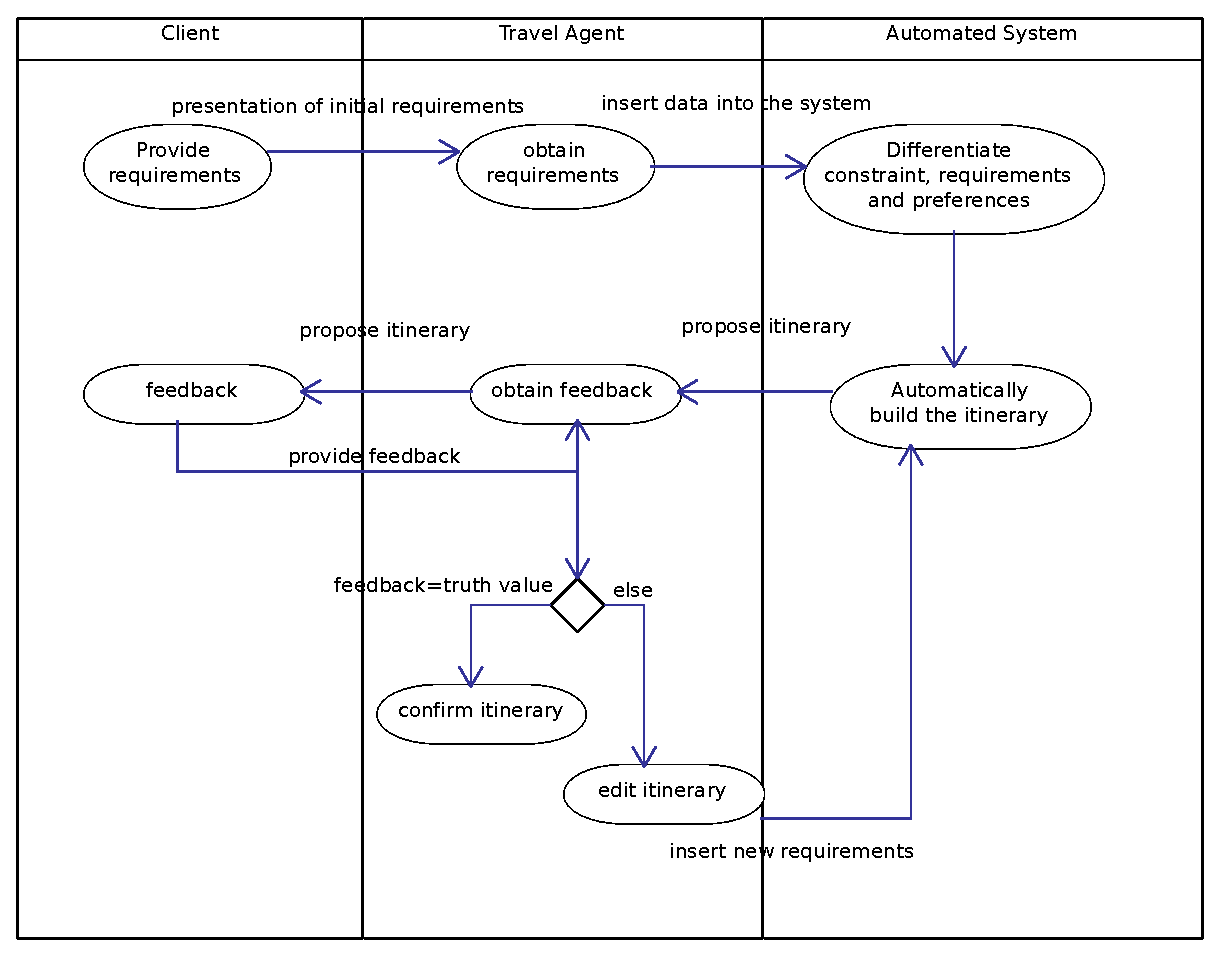
\includegraphics[width=\textwidth]{images/communication.eps}
\caption{Communication process}
\label{fig:CommunicationDiagram}
\end{figure}

\worksheet{CM-1}{Transaction Descritpion worksheets}

\worksheet{CM-2}{Information exchange specification}

\clearpage
\section{Design Knowledge}

\worksheet{DM-1}{System Architecture}

\worksheet{DM-2}{Target implementation platform}

\newpage
\section{Implementation}
To implement the system in order to create a portable, scalable and user-friendly application it has been decided to develop a web-based service in Python with a basic GUI using HTML, CSS and Javascript (jQuery framework).\\
\indent As the client/server communication is based on AJAX and standard HTTP requests, we exploited the functionalities provided by the Flask framework for pyhton. Additionally, we adopted an ulterior Python framework, SQLAlchemy, to manage the communicaton between the application and the database.\\
\indent The basic setup of the final system is built as follows:
\begin{description}
\item[GUI] \hfill \\
The user interface needs to be user friendly and easy to use, so to prevent the necessity of additional training for the Travel Agent that interacts directly with it. Built as a standard webpage, the GUI provides the TA with an extremely easy-to-use panel where to insert the information provided by the client such as: start date and end date of the planned trip, the presence of kids, the need for free time (time not filled in by the TA to be able to roam freely around the city), the customer's preference for quiet environments, the customer's willingness to walk long distances, and his preferences regarding four types of attractions (shopping, culture, gastronomy or night-life).\\
Once the TA has filled in the necessary information, can request the itinerary to the system by simply clicking the \textit{Next} button. The interface will then show a list of the locations chosen for each day, which can be furtherly modified by the travel agent. By chosing to edit the itinerary, it will in fact be offered the opportunity to exclude some locations that do not satisfy the customer's desires. These modifications will then be forwarded to the system that will provide a new itinerary to show.\\
If the customer is satisfied with the proposed itinerary, then the TA can confirm the choice and end the procedure.
\item[Server Side] \hfill \\
The back-end consists in the set of rules and functions that constitute the server-side of the application. It has been neatly divided using a model-view-controller approach as illustrated in the previous diagrams, and provides functionalities of communication with the database, communication with the front-end, and a ``knowledge engine" embedding the TA knowledge necessary to build the itinerary.\\
The entire server-side application has been build on the base of the inference model designed in the previous part of the document, and will be explained further in Section \ref{sec:common}.
\item[Database] \hfill \\
The SQL based database contains the information relative to the client and the locations that will be handled by the ``knowledge engine" to build the itinerary. The database has been build on the base of the domain model in Section \ref{sec:domain}, and has been filled with information coming directly from the \textit{TripAdvisor} database. This specific way of building and filling the database favours the reusability of the whole application (for more information see Section \ref{sec:reusability})
\end{description}

\subsection{Knowledge inside the software}
The three types of rules designed for our system (constraint-rules, preference-rules, requirement-rules) have been implemented in the function \textit{selectLocation()}. The rules have been implemented as a series of SQL queries to the database to carefully select the right locations, with the aid of a probability function, needed to implement the connector \textit{prefers-with-probability} (see Section \ref{sec:rules}).


\subsection{Role of the CommonKADS model set in the implementation} \label{sec:common}
The implementation of the system was strongly based on the models prepared in the previous sections of this document, particularly on the Inference Model in section \ref{sec:inference} and the Domain Model in section \ref{sec:domain}.\\
In this section it is illustrated briefly the correspondence between the functions implemented in \textit{easyAround} and the roles and transfer functions of the inference model.
\subsubsection{Roles}
In the implementation of the software it is possible to recognize some data structures or classes that constitute the main entities of the system; each of these classes or data structures corresponds to an Inference Role. In this section it is presented a list of these data structures, complete of their role inside the Inference model and a brief explanation.
\begin{description}
\item[Request] \hfill \\
Inference Role: request;\\
This is the class that contains the initial request coming from the customer, and represents the starting point of the whole system.
\item[Skeletal Design] \hfill \\
Inference Role: skeletal design;\\
This data structure is an aggregation of the days the itinerary is composed of, and needs to be later filled with appropriate locations. It constitutes the ``skeleton'' of a complete itinerary.
\item[Preferences, Requirements and Constraints] \hfill \\
Inference Role: preferences and requirements, constraints;\\
These three data structures contain the information needed to correctly classify the needs of the customer and build an itinerary accordingly.
\item[Itinerary] \hfill \\
Inference Role: proposal, itinerary;\\
This data structure constitutes the final itinerary, composed of all the days and the locations. It can be accepted by the customer, or rejected with new directives, and in this case it undergoes modifications.
\end{description}
The roles in the inference not shown in this list have been implemented as much simpler data structures such as lists or arrays, and are: \textit{violation, customer input, action list, action}.
\subsubsection{Transfer Functions}
The methods implemented in the software have, as well as classes and data structures, a unique correspondence to the Inference model. In this section is presented the list of the main methods implemented, complete of their role inside the Inference model and a brief explanation.
\begin{description}
\item[Specify(request)] \hfill \\
Function: specify;\\
Creates the basic structure of the itinerary, the skeletal design.
\item[Operationalize(request)] \hfill \\
Function: operationalize;\\
Divides all the parameters in requirements, preferences and constraints.
\item[Propose(requirements, preferences, constraints, skeletal design)] \hfill \\
Function: propose;\\
Builds the itinerary based on the request of the client, using the knowledge rules.
\item[Verify(proposal)] \hfill \\
Function: verify; \\
Submits the itinerary to the client.
\item[Critique(violation, itinerary)] \hfill \\
Function: critique;\\
Edits the itinerary accordingly to the critique obtained from the client.
\item[Select(location, itinerary)] \hfill \\
Function: select;\\
For each violation, selects one single action to be performed and passes the control to modify.
\item[Modify(constraints)] \hfill \\
Function: modify;\\
Takes the selected action and commits the modification into the database.
\end{description}


\subsection{Reflection on problems and results}

The result of this project is a piece of software that represents a first completely functioning version of what could be a much broader system for travel planning. We consider ourselves satisfied with the result as the usability and the functionality of the software is coherent with the initial objectives, even though during the development process we encountered some difficulties.

The idea of developing a software in this domain was supported by the fact that knowledge is largely avaiable: information can be found on the Internet and even extracted from common sense notions (for example the fact that elderly people should not go climbing mountains). Thanks to this fact we were able to develop an efficient system without bothering too much our expert, who remained avaiable for important matters and maintained a very positive attitude towards us.\\
The avaiability of knowledge implies that data is easily is retrievable from any online database, complete with all the attributes needed to build an efficient knowledge engine. This made our job easier because we could avoid manually inserting all the data into the system.

One of the problems we faced was the broadness of the domain. Although we started by restricting it to a single city, the quantity of variables to be considered in selecting a solution remained huge. To be able to present a "minimum viable product" (MVP) able to provide basic functionalities, we adopted a spiral approach where we considered just the most important factors (extracted from a second interview with the expert) excluding complicated variables like monetary costs. 

In the early stages of software development we realized that one of the objectives was too ambitious: we intended to offer an itinerary where the distances between the locations were calculated according to the customers' needs. However we soon realized that given the time and resources, the task was too complicated. The problem was analogous to the Travelling Salesman Problem (TSP) which unfortunately is NP-complete~\cite{papadimitriou1977euclidean}. We decided to avoid partial or over-simplified solutions (randomly choosing a combination of locations leaving the eventual check to the TA), and simply move these features in a more advanced level of the spiral (See section~\ref{sec:spiral}).

During the implementation phase we also realized that the select-modify cycle inside the inference model template "configuration design" could have been optimized and that it did not reflect precisely the needs of our software. However we decided to remain coherent to the original template, in order to exploit the reliability of a standard model.

During the whole project one of the most time expensive task was to keep the documentation syncronized with the actual implementation. Despite the fact that it was a feasible task for two people, it would have been more difficult for a larger group.

We also realized the importance of calculating the risks before starting the actual development. Despite the careful designing of the models and the scheduling we constructed for the implementation, we did not consider risks related to human components of the project: the testing phase of the software was delayed of almost four days.


\subsubsection{Spiral Approach}\label{sec:spiral}
In this section is illustrated how the various models designed for this project can be expanded in the next phase of the spiral. By adding the functionalities relative to distance calculations, we can also demonstrate how easy it is to apply modifications to the already functioning product without disrupting its internal structure.

\myparagraph{Inference Knowledge} 


\noindent
\begin{tabular}{|p{2cm}|p{3cm}|p{3cm}|p{6cm}|}
  \hline
Inference   & Input & Output  & Description \\ \hline \hline
specify   & request & skeletal design   & the function builds the default skeletal design: the basic structure of a trip where each day is composed of: an heavy activity during the morning, a relaxing afternoon, evening and meal.
\\ \hline
\end{tabular}

\myparagraph{Domain schema}

The domain schema can be found in Figure~\ref{fig:ClassDiagram2}


\begin{description}
  \item[Client] \hfill \\
  The client who goes to the travel agency. He can express preferences for a quiet enviroment and express his willingness to travel long distances by foot (\emph{dynamic}). The clients are categorized by their age to avoid unsuitable locations (ex: elderly people in a climbing location).

\item[Location] \hfill \\
  This model represents the point of interests that a customer could visit. The attribute \emph{rating} describes the quality of this place, \emph{intensive} describes if the place is not for quite people and \emph{excludedCategory} specifies if a client category is not suitable for the location (ex: elderly people in a climbing location). The method \emph{distance} takes two locations and returns the distance between them. It is useful in order to create the combination of locations to visit during a trip.
\end{description}

\myparagraph{Rule types}

\begin{lstlisting}[label=Rules,caption=The client is a quite person,breaklines=true,mathescape=true]
client.quiet=true, client.needsFreeTime=true, client.active=1
REQUIRES
itinerary.day.timeslot.location, location.intensive=false;
itinerary.day.timeslot, timeslot.location=NULL;
$\sum_{i=1}^{n-1}$i.distance(i+1) $<\delta$, $\forall$i $\in$ location;
\end{lstlisting}

\begin{figure}[H]
\centering
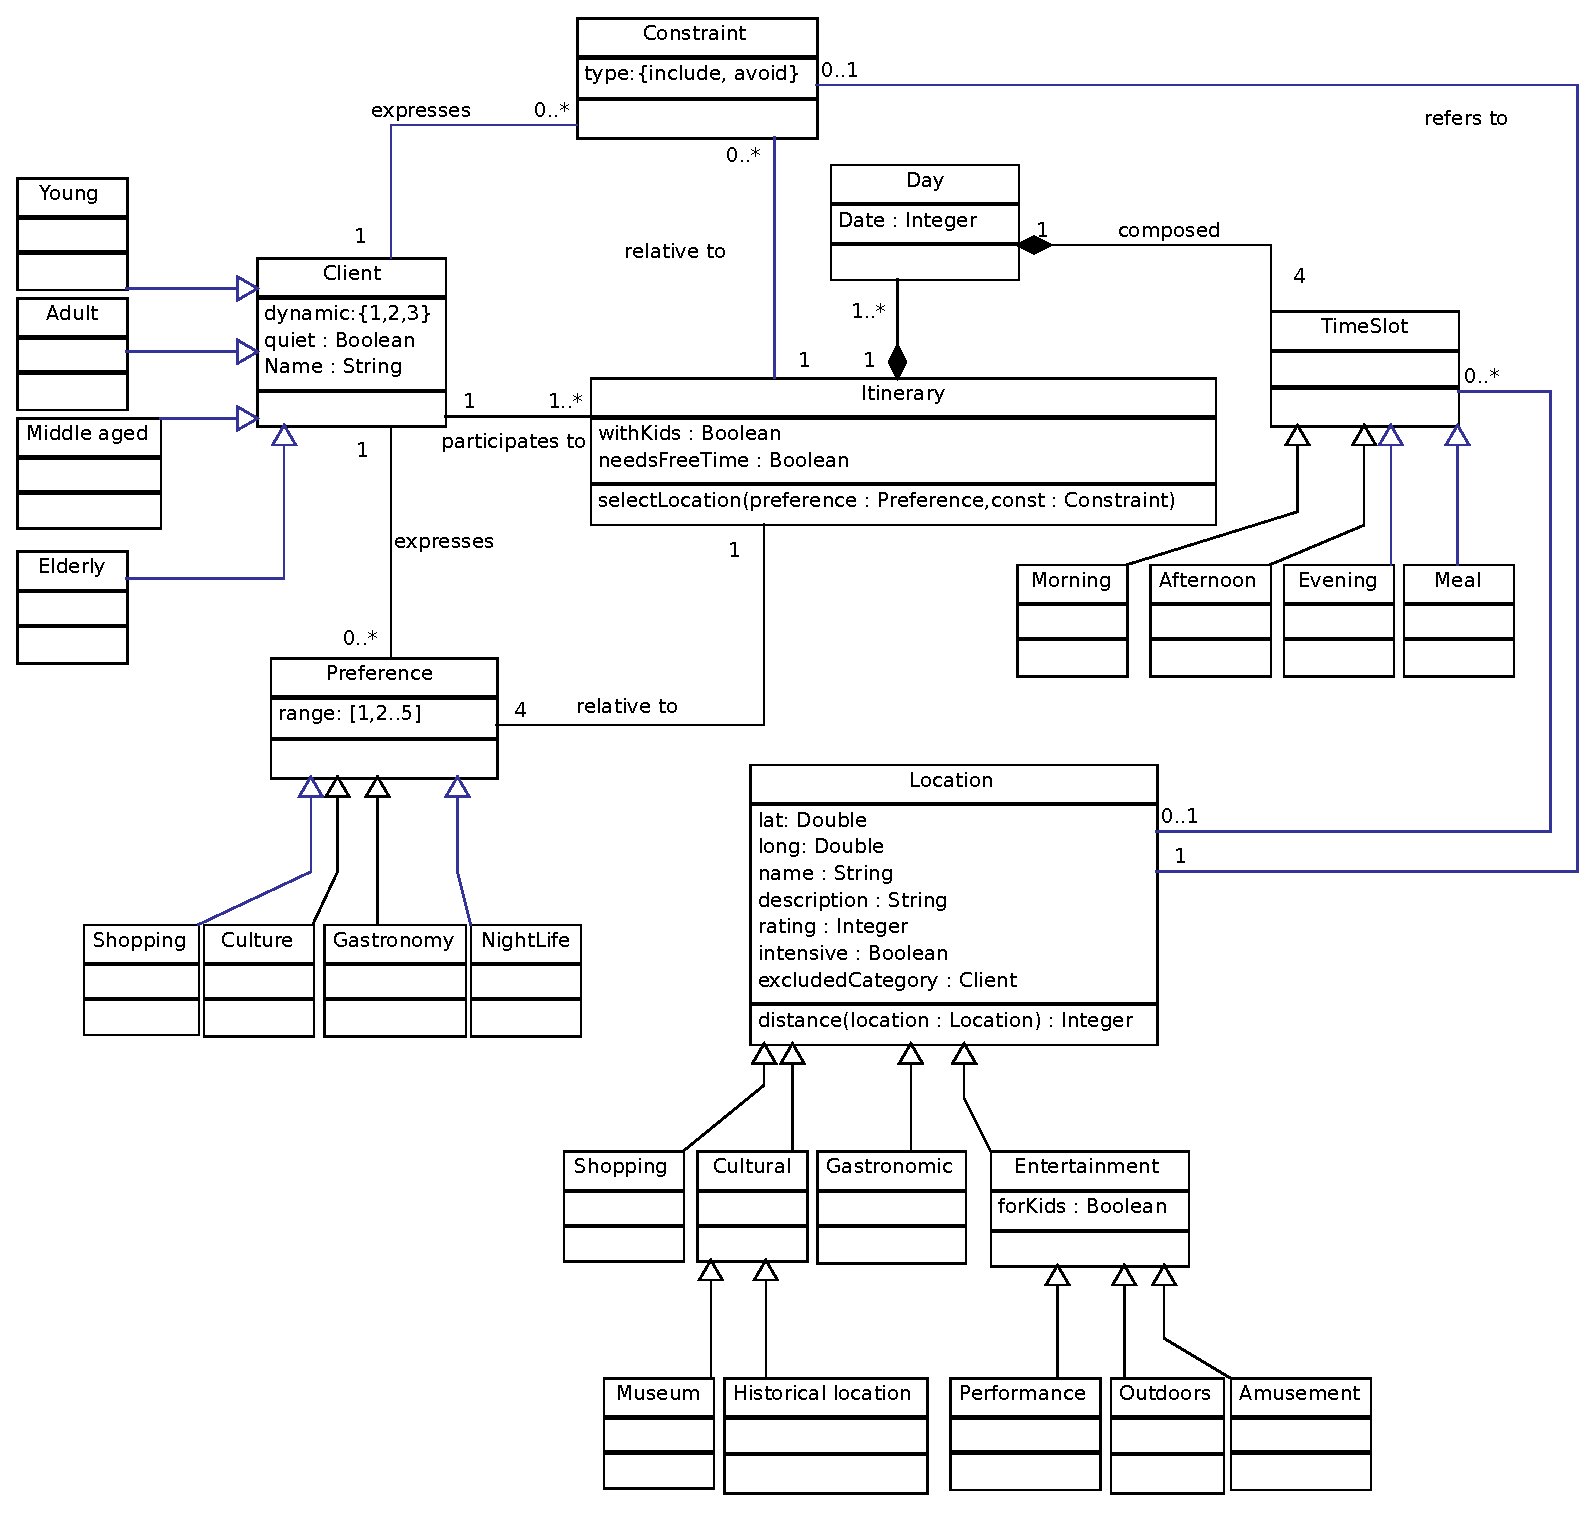
\includegraphics[width=\textwidth]{images/domain.eps}
\caption{Domain schema}
\label{fig:ClassDiagram2}
\end{figure}
\newpage
\myparagraph{Communication Knowledge}
\worksheet{CM-2a}{Information exchange specification}



\subsection{Reusability} \label{sec:reusability}
The application was build to be completely reusable, making sure that the choice of a restricted domain (the city of Rome) would not influence the performance of the system itself.\\
\indent If, for example, the travel agency is interested in focusing the choice of points of interest on Amsterdam instead of Rome, the only thing that would be subjected to change is the data inside the database. The construction of the database itself and the whole application are absolutely not domain dependant, so they will automatically adapt the choice for the new itinerary on the available data, independently from its origin. The only action that needs to be performed in this case is just the one that recovers the data from the \textit{TripAdvisor} database (or any other tourism-related database) accordingly to the need of the application.\\
\indent This can be possible thanks to the generality of the rules in the \textit{knowledge engine}, that base the choice of points of interest not on the locations themselves, but on the category to which they belong: a location dedicated to culture like a museum is easily recognizable both in Amsterdam and in Rome, even if the theme or purpose of that specific location are different. For example, \textit{Van Gogh Museum} in Amsterdam and \textit{Museo Civico di Zoologia} in Rome have nothing in common, but the application is able to suggest both to a person interested in culture.\\
\indent Note however that the data inside the database \textit{must} be complete of all the necessary information: if a location is not correctly classified (for example its coordinates are not known or its category is not specified) the application will not be able to perform at its full capacity.

\subsection{Code distribution}
In order to have a public example of a project developed on the commonKADS methodologies, the system is Open Source distributed and it can be retrived at \url{https://github.com/denadai2/EasyAround.git}

\newpage

\appendix
\section{Design Knowledge}

In preparation for the interview with the expert we listed a series of concepts to be clarified in order to better structure the application domain. 

\begin{enumerate}
  \item Target of the application: which kind of customer the application is more suitable for;
  \item Subcategories of the target: is it possible to recognize different subcategories in the target that correspond to different needs for the creation of an itinerary;
  \item Locations of interest: understand which categories of locations can be created and in which way they can be matched with the customer's preferences;
  \item Composition of the itinerary: understand the basic structure of an itinerary, and whether it can be composed automatically.
\end{enumerate}

The interviewing techniques applied were mainly two: problem solving (the interviewer poses himself as a customer and watches the expert ``in action") and 20-Questions (the interviewer thinks about a destination for an hypothetical itinerary and the expert needs to guess which one it is). Relatively to the categorization of the locations, it has also been used the ``Card sorting".
The results of the interview were satisfying:

\begin{enumerate}
  \item The target of the application are the ``lonely travelers", people who prefer traveling on their own, at most with their family.
  \item It has been concluded that the target can be divided in four age-based category, such as ``Young" (18-30), ``Adults" (30-40), ``Middle aged" (40-60), ``Elderly" (60+). Relating to these categories the aspects that change the most are: need for entertainment, need for quiet, free time available, amount of time spent walking.
  \item The locations can be divided in four main categories such as ``shopping", ``gastronomy", ``cultural" and ``entertainment"; of these, ``cultural" can be divided in ``historical locations" (such as monuments) and ``museums", and ``entertainment" can be divided in ``amusement" (such as clubs, pubs and discos), ``performance" (such as cinemas, theatres, \ldots)  and ``outdoor" (such as amusement parks or gardens).
  \item It has been concluded that the itinerary can be seen as an aggregation of days, which in turn have a basic fixed structure. 
\begin{description}
  \item[Morning] non intensive activity (monuments, gardens\ldots);
  \item[Afternoon] intensive activity (museums, shopping\ldots);
  \item[Evening] the intensity of the activity depends on personal preferences.
\end{description}
\end{enumerate}

From the interview emerged an aspect not considered before, that is to say the presence of kids. The expert pointed out that in case a child is present, the itinerary is to be built as usual but having care of including children activities every once in a while.
A constraint to be considered is the fact that the customer can request a location to be included or excluded from the itinerary.


\nocite{*}
\bibliographystyle{amsplain}
\bibliography{biblio}


\end{document}
